\documentclass[journal]{IEEEtran}
\usepackage[superscript,nocompress]{cite}
\renewcommand{\citepunct}{,}
\usepackage{amsmath}
\usepackage{graphicx}
\usepackage{booktabs}
\usepackage{array}
\usepackage{tikz}
\usetikzlibrary{positioning,arrows.meta}
\usepackage{xurl}
\usepackage[hidelinks]{hyperref}
% Generated by experiments/make_numbers.py from results/*.json. Do not edit.
\newcommand{\LifeDays}{1{,}826}
\newcommand{\ResSLCmin}{26}
\newcommand{\ResPSLCh}{2.2}
\newcommand{\ResPSLCHighh}{1.5}
\newcommand{\ResTLCh}{14.6}
\newcommand{\ResQLCh}{43.8}
\newcommand{\DwpdSLC}{55}
\newcommand{\DwpdTLC}{1.6}
\newcommand{\DwpdQLC}{0.55}
\newcommand{\RatioTLC}{11.1}
\newcommand{\RatioQLC}{25}
\newcommand{\RatioPSLC}{5}
\newcommand{\WriteAllLlamaTB}{513}
\newcommand{\WriteAllDSTB}{110}
\newcommand{\KVRatio}{4.66}
\newcommand{\ShareSLCLlama}{46.9}
\newcommand{\ShareTLCLlama}{4.2}
\newcommand{\ShareQLCLlama}{1.9}
\newcommand{\LifeSLCLlama}{2.35}
\newcommand{\LifeTLCLlama}{0.21}
\newcommand{\BudgetSLCNodeTB}{241}
\newcommand{\BudgetTLCNodeTB}{21.7}
\newcommand{\RecN}{11}
\newcommand{\RecPapers}{3}
\newcommand{\SameDieMin}{2.2}
\newcommand{\SameDieMax}{3.3}
\newcommand{\SameDieHundred}{11.1}
\newcommand{\RecMin}{0.75}
\newcommand{\RecMax}{20}
\newcommand{\RecFiveY}{6}
\newcommand{\RecWafTwoFiveY}{4}
\newcommand{\RecTLCFiveY}{0}
\newcommand{\RecTLCMax}{1.8}
\newcommand{\RecQLCMax}{0.8}
\newcommand{\RecGainMin}{2.8}
\newcommand{\RecGainMax}{74}
\newcommand{\RecDwpdMin}{13}
\newcommand{\RecDwpdMax}{365}
\newcommand{\TLCFactor}{0.09}
\newcommand{\QLCFactor}{0.04}
\newcommand{\YuAwareTLC}{1.33}
\newcommand{\BaekEvictTLC}{1.80}
\newcommand{\GapWindowMin}{30}
\newcommand{\QwWindowMin}{90}
\newcommand{\QwSlcMin}{74}
\newcommand{\QwSlcMax}{95}
\newcommand{\QwAfterMin}{5}
\newcommand{\QwAfterMax}{26}
\newcommand{\QwReuseMin}{2.1}
\newcommand{\QwReuseMax}{28}
\newcommand{\QwMedMin}{6.1}
\newcommand{\QwMedMax}{7.9}
\newcommand{\MoReuseMin}{2}
\newcommand{\MoReuseMax}{28}
\newcommand{\MoReuseDSMin}{4.8}
\newcommand{\MoReuseDSMax}{8.4}
\newcommand{\WcFollowUps}{300{,}083}
\newcommand{\WcMedianS}{112}
\newcommand{\WcOverOneH}{4.4}
\newcommand{\WcOverFifteenH}{0.62}
\newcommand{\WcOverDay}{0.27}
\newcommand{\TlMeanMin}{46.7}
\newcommand{\TlMedianMin}{1.4}
\newcommand{\TRecMs}{64}
\newcommand{\TDramMs}{2.7}
\newcommand{\ValueDramMs}{2.6}
\newcommand{\TSsdMs}{21}
\newcommand{\THbfUs}{26}
\newcommand{\THbfOneUs}{105}
\newcommand{\ValueRatio}{24}
\newcommand{\ValueRatioDS}{60}
\newcommand{\SsdShareOne}{6.2}
\newcommand{\SsdShareThree}{18.7}
\newcommand{\SsdResThreeH}{8}
\newcommand{\BlockMiB}{160}
\newcommand{\RegimeP}{26}
\newcommand{\TLCBudgetStack}{2.7}
\newcommand{\QLCBudgetStack}{1.2}
\newcommand{\SLCBudgetStack}{30}
\newcommand{\LlamaReusableStack}{16.5}
\newcommand{\LlamaOverTLC}{6.1}
\newcommand{\DSReusableStack}{0.66}
\newcommand{\DSOverTLC}{0.24}
\newcommand{\LlamaIdealSLC}{92}
\newcommand{\LlamaIdealTLC}{16}
\newcommand{\LlamaRandSLC}{41}
\newcommand{\LlamaRandTLC}{4.2}
\newcommand{\DSIdealSLC}{100}
\newcommand{\DSIdealTLC}{100}
\newcommand{\DSRandSLC}{94}
\newcommand{\DSRandTLC}{20}
\newcommand{\RegimeMargin}{5}
\newcommand{\SlcAheadMin}{22}
\newcommand{\SlcAheadMax}{24}
\newcommand{\QlcAheadMin}{11}
\newcommand{\QlcAheadMax}{22}
\newcommand{\PSLCBudgetStack}{6.0}
\newcommand{\SigmaFit}{2.30}
\newcommand{\WcOverTLC}{0.64}
\newcommand{\DwpdRatioMin}{0.2}
\newcommand{\DwpdRatioMax}{6.7}
\newcommand{\SLCOverTLCDwpd}{33}
\newcommand{\YuCutMin}{12}
\newcommand{\YuCutMax}{14}
\newcommand{\SimNodeGPUh}{192}
\newcommand{\SimRoarSLC}{5.8}
\newcommand{\SimRoarTLC}{2.6}
\newcommand{\SimRoarSSD}{5.3}
\newcommand{\SimRoarSLCpct}{3.0}
\newcommand{\SimRoarTLCpct}{1.4}
\newcommand{\SimSlcOverTlc}{2.2}
\newcommand{\SimOracleOverRoarMin}{1.7}
\newcommand{\SimOracleOverRoarMax}{2.1}
\newcommand{\SimRoarOverAkMin}{6}
\newcommand{\SimRoarOverAkMax}{14}
\newcommand{\SimWaSLC}{3.9}
\newcommand{\SimWaTLC}{0.5}
\newcommand{\SimAkTLC}{2.5}
\newcommand{\SimTlcPolicySpread}{5}
\newcommand{\SimConvRoarSLC}{6.0}
\newcommand{\SimConvRoarTLC}{2.4}
\newcommand{\SimNoDramRoarSLC}{10.5}
\newcommand{\SimNoDramRoarTLC}{4.5}
\newcommand{\SimDramTwoRoarSLC}{3.3}
\newcommand{\SimDramFourRoarSLC}{1.0}
\newcommand{\SimDramTwoRoarTLC}{1.7}
\newcommand{\SimDramFourRoarTLC}{0.9}
\newcommand{\SimWafTwoRoarSLC}{5.0}
\newcommand{\SimWafTwoRoarTLC}{2.1}
\newcommand{\WcReturnPct}{2.8}
\newcommand{\SimDsRoarSLC}{0.50}
\newcommand{\SimDsRoarTLC}{0.72}
\newcommand{\SimDsRoarSSD}{1.93}
\newcommand{\SimDsSecondSLC}{0.72}
\newcommand{\SimDsOracleOverRoarMax}{4.7}
\newcommand{\SimDsWaShare}{46}
\newcommand{\SimDsSlcResMin}{56}
\newcommand{\SimOracleWrittenMax}{58}
\newcommand{\SimMaxOver}{56}
\newcommand{\SimRetXZeroSLC}{5.5}
\newcommand{\SimRetXZeroTLC}{1.9}
\newcommand{\SimRetXZeroRatio}{2.8}
\newcommand{\SimRetXFourSLC}{6.2}
\newcommand{\SimRetXFourTLC}{3.9}
\newcommand{\SimRetXFourRatio}{1.6}
\newcommand{\SimWafTwoDropSLC}{14}
\newcommand{\SimWafTwoDropTLC}{21}
\newcommand{\SimCeilZero}{19.8}
\newcommand{\SimCeilOne}{12.1}
\newcommand{\SimCeilTwo}{8.1}
\newcommand{\SimCeilFour}{4.4}
\newcommand{\SimCeilFourPct}{2.3}
\newcommand{\SimCeilDS}{2.39}
\newcommand{\SimDramShareOne}{39}
\newcommand{\SimDramShareTwo}{59}
\newcommand{\SimDramShareFour}{78}
\newcommand{\SimNoDramSlcShare}{53}
\newcommand{\SimRoarSlcCeilPct}{48}
\newcommand{\SimRoarTlcCeilPct}{22}
\newcommand{\SimRoarSsdCeilPct}{44}
\newcommand{\SimOracleSlcCeilPct}{82}
\newcommand{\SimOracleSLC}{9.9}
\newcommand{\SimOracleSSD}{10.5}
\newcommand{\SimDramFourAkSLC}{0.9}
\newcommand{\SimDramFourAkTLC}{0.8}
\newcommand{\SimHitsPerBlockSLC}{0.18}
\newcommand{\SimHitsPerBlockTLC}{0.87}
\newcommand{\SimReusableL}{72}
\newcommand{\SimReusableDS}{3.6}
\newcommand{\SimReusableLOverTLC}{3.3}
\newcommand{\SimReusableLOverSLC}{0.30}
\newcommand{\SimReusableDSOverTLC}{0.17}
\newcommand{\SimPslcOverTlcPct}{37}
\newcommand{\SimPslcOverTlcAkPct}{28}
\newcommand{\SimWriteBwRatio}{23}
\newcommand{\SimReusableLOverSLCPct}{30}
\newcommand{\SimReusableDSOverTLCPct}{17}
\newcommand{\SimWafTwoDropRangeSLC}{14--19}
\newcommand{\SimWafTwoDropRangeTLC}{21--26}
\newcommand{\SimSsdHitValuePct}{96}
\newcommand{\DramBiasPct}{4}
\newcommand{\SimEnduranceGBs}{0.35}
\newcommand{\SimDramGBsOne}{0.7}
\newcommand{\SimDramLinkPctOne}{1}
\newcommand{\SimDramGBsFour}{1.3}
\newcommand{\SimDramLinkPctFour}{2}
\newcommand{\DramResLs}{91}
\newcommand{\DramResDSmin}{10}
\newcommand{\DramShareL}{41}
\newcommand{\DramShareDS}{97}
\newcommand{\SimRoarOverMax}{56}
\newcommand{\SimAkOverMax}{2}
\newcommand{\SimRoarOverShown}{18}
\newcommand{\SimDsAkTLC}{0.76}
\newcommand{\SimDsAkSSD}{1.69}
\newcommand{\SimDsOracleMin}{2.37}
\newcommand{\SimDsOracleMax}{2.39}
\newcommand{\SimDramFourRoarOverPct}{18}
\newcommand{\SimDsWrittenPct}{47}
\newcommand{\SimDsSsdOverPct}{15}
\newcommand{\SimRetXSixteenSLC}{6.6}
\newcommand{\SimRetXSixteenTLC}{6.5}
\newcommand{\SimRetXSixteenRatio}{1.0}
\newcommand{\SimXFourDramShareFour}{56}
\newcommand{\SimXFourFourSLC}{1.3}
\newcommand{\SimXFourFourTLC}{1.8}
\newcommand{\SimXFourCeilFour}{12.7}
\newcommand{\SimSeedSpreadMax}{4}
\newcommand{\SimSeedRatioMin}{2.2}
\newcommand{\SimSeedRatioMax}{2.2}
\newcommand{\SimSeedRatioRange}{2.2}
\newcommand{\SimSeedDsSlcMin}{0.71}
\newcommand{\SimSeedDsSlcMax}{0.72}
\newcommand{\SimSeedDsTlcMin}{0.76}
\newcommand{\SimSeedDsTlcMax}{0.76}
\newcommand{\SimSeedDsSsdMin}{1.74}
\newcommand{\SimSeedDsSlcRange}{0.71--0.72}
\newcommand{\SimSeedDsSsdAkRange}{1.63--1.72}
\newcommand{\SimSeedDsTlcRange}{0.76}
\newcommand{\SimRelaxTlcL}{4.1}
\newcommand{\SimPslcHighL}{3.9}
\newcommand{\SimRelaxTlcDS}{1.05}
\newcommand{\YuPlainCutMin}{1.4}
\newcommand{\YuPlainCutMax}{3.9}

\makeatletter\newcommand{\tabinput}[1]{\@@input #1 }\makeatother
\newcommand{\hd}[1]{\begin{tabular}[b]{@{}c@{}}#1\end{tabular}}
\newcommand{\repourl}{\url{https://github.com/ho3nik/hbf-endurance}}
\graphicspath{{../figures/}}

\begin{document}
\bstctlcite{IEEEexample:BSTcontrol}

\title{Host DRAM First: What High Bandwidth Flash Adds to an LLM KV Cache}

\author{H.~R.~J.~Nikzat, Bates College}

\maketitle

\begin{abstract}
High Bandwidth Flash (HBF) stacks NAND flash next to an AI accelerator, and several 2026 papers propose keeping the key--value (KV) cache of LLM or recommendation serving on it. They report lifetimes from \RecMin{} to \RecMax{} years. In drive writes per day, their workloads ask for \RecDwpdMin{} to \RecDwpdMax{}, while a five-year single-level-cell (SLC) stack sustains \DwpdSLC{}. Written at its five-year budget, an SLC stack keeps each block for \ResSLCmin{} minutes and a triple-level-cell (TLC) stack for \ResTLCh{} hours; on TLC, none of these designs lasts five years. We then simulate an eight-GPU node. Host DRAM takes most of the value: 4~TB of it recovers \SimDramShareFour{}\% of what an unlimited cache below HBM could. Behind 1~TB of DRAM, SLC flash saves \SimRoarSLC{} of \SimNodeGPUh{} GPU-hours per day and TLC \SimRoarTLC{}. For a compact KV format, the cell type barely matters and an SSD pool saves more.
\end{abstract}

\begin{IEEEkeywords}
High bandwidth flash, NAND flash endurance, KV cache, LLM inference, memory hierarchy.
\end{IEEEkeywords}

\IEEEPARstart{H}{igh} Bandwidth Flash (HBF) is NAND flash stacked on a logic die and placed next to an accelerator, the way High Bandwidth Memory (HBM) stacks DRAM. The first open specification, released through the Open Compute Project in August 2026, allows up to 512~GiB per stack and read bandwidth between about 0.4 and 3.0~TB/s.\cite{ocp2026hbf} One stack holds several times what an HBM stack holds. That makes HBF a candidate home for the largest memory consumer in LLM serving: the key--value (KV) cache.

The KV cache holds, for every token a model has processed, the attention keys and values that later tokens read. Serving systems keep it after a request ends, because many conversations and agent sessions come back and reuse the same prompt prefix. Flash has a cost here that DRAM does not. Each NAND cell survives only a rated number of program/erase cycles, so every block written to flash uses up part of its life, whether or not the block is read again.

Papers that put KV caches on HBF disagree on how long the flash lasts. Yu et al.\ report 1.21 to 14.82 years for the same hardware under three request-scheduling policies, which decide which requests run and how much device memory they may hold.\cite{yu2026hbf} Baek et al.\ report 8 to 20 years,\cite{baek2026hotcold} and Peng et al., for recommendation serving, about one year under least-recently-used (LRU) replacement and over six with a filter that admits a block only after $K=10$ references.\cite{peng2026gr} Li et al.\ model denser cells and compare an HBF tier with an SSD pool of equal capacity for KV-cache offloading; the HBF tier wears out first.\cite{li2026hbfsucks} Still open is how much GPU time HBF saves once host DRAM and SSDs, which a serving node already has, can hold the same blocks.

This article answers both questions for architects who know flash or LLM serving but not both. It makes four points.
\begin{enumerate}
\item Converted to drive writes per day, the published lifetimes can be set against what each cell type sustains. Residence time, how long a flash log keeps a block before overwriting it, shows what a denser cell changes. Every lifetime we can recompute assumes SLC, and none lasts five years on TLC.
\item On public two-hour traces, up to about a quarter of KV reuse arrives after SLC has discarded the block.
\item In a simulated eight-GPU node, 2 to 4~TB of host DRAM, what a DGX B200 ships with or supports, recovers most of what an unlimited cache below HBM could. How much flash adds, and which cell type wins, depends on the reusable write rate: the bytes per day that leave DRAM and will be read again. An SSD pool is a strong alternative.
\item Lifetime claims become comparable when papers report a short list of inputs, given at the end.
\end{enumerate}
Code that regenerates every number, table and figure is open at \repourl.

\section{KV caches and flash wear}

\emph{KV state per token.} Llama-3.1-70B stores 327,680 bytes per token: a key and a value vector of 128 two-byte numbers for each of its 8 key--value heads in each of 80 layers. DeepSeek-V3 compresses each layer's KV state into one shorter vector and stores 70,272 bytes per token, \KVRatio{} times less. Serving systems handle KV state in fixed blocks; a block of 512 Llama-3.1-70B tokens is \BlockMiB{}~MiB.

\emph{Prefix reuse.} With prefix caching, each block is named by a hash of every token up to its end. A cached block helps a request only if every earlier block of its prompt is also cached. When HBM is full, the serving system evicts blocks, usually the least recently used. An evicted block can go to host DRAM, to SSDs, or to HBF, or it can be dropped and recomputed later. Mooncake, for example, builds its serving system around a KV store in host memory and SSDs.\cite{qin2025mooncake} Fig.~\ref{fig:tiers} shows the hierarchy we simulate and what each tier costs when a block is needed again.

\begin{figure}[t]
\centering
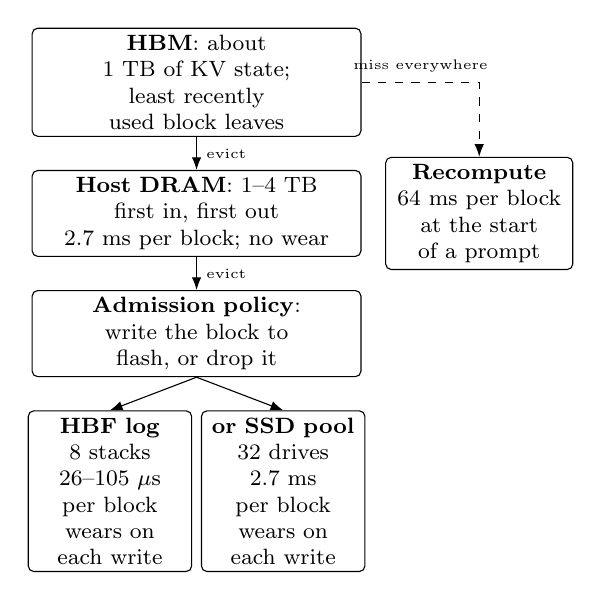
\begin{tikzpicture}[font=\footnotesize, box/.style={draw, rounded corners=2pt, align=center, inner sep=2.5pt},
  arr/.style={-{Latex[length=1.6mm]}, thin}]
\node[box, text width=4.0cm] (hbm) {\textbf{HBM}: about 1~TB of KV state;\\least recently used block leaves};
\node[box, text width=4.0cm, below=0.42cm of hbm] (dram) {\textbf{Host DRAM}: 1--4~TB\\first in, first out\\\TDramMs{}~ms per block; no wear};
\node[box, text width=4.0cm, below=0.42cm of dram] (adm) {\textbf{Admission policy}:\\write the block to flash, or drop it};
\node[box, text width=1.9cm, below=0.42cm of adm, xshift=-1.1cm] (hbf) {\textbf{HBF log}\\8 stacks\\\THbfUs{}--\THbfOneUs{}~$\mu$s per block\\wears on each write};
\node[box, text width=1.9cm, below=0.42cm of adm, xshift=1.1cm] (ssd) {\textbf{or SSD pool}\\32 drives\\\TDramMs{}~ms per block\\wears on each write};
\node[box, text width=2.2cm, right=0.3cm of dram] (rec) {\textbf{Recompute}\\\TRecMs{}~ms per block at the start of a prompt};
\draw[arr] (hbm) -- node[right, font=\tiny]{evict} (dram);
\draw[arr] (dram) -- node[right, font=\tiny]{evict} (adm);
\draw[arr] (adm.south) -- (hbf.north);
\draw[arr] (adm.south) -- (ssd.north);
\draw[arr, dashed] (hbm.east) -| node[above, pos=0.25, font=\tiny]{miss everywhere} (rec.north);
\end{tikzpicture}
\caption{The KV-cache hierarchy we simulate, with the time to bring back one Llama-3.1-70B block from each tier. Times assume 1.6~TB/s per HBF stack (one stack to four striped), 63~GB/s of PCIe bandwidth and 8~GB/s per SSD,\cite{yu2026hbf} and, for recomputation, twice the active parameters (141.2~GFLOP) per token plus attention, on a B200 at half its 2.25~PFLOP/s peak.}
\label{fig:tiers}
\end{figure}

\emph{The HBF device.} Endurance, not write bandwidth, limits how much a stack can write. To last five years, eight SLC stacks can write \BudgetSLCNodeTB{}~TB per day. That is \SimEnduranceGBs{}~GB/s per stack, about \SimWriteBwRatio{} times less than the 8~GB/s of write bandwidth Yu et al.\ assume.\cite{yu2026hbf} Reads take microseconds. We assume 1.6~TB/s of read bandwidth per stack, inside the specification's range.

\emph{Wear.} A flash cell stores bits as charge, and each program/erase cycle wears the oxide that holds it. Cells that store more bits wear out sooner. Industry figures put single-level cells (SLC, one bit) at up to 100,000 cycles and 3D triple-level cells (TLC, three bits) at 3,000. Pseudo-SLC (pSLC, a multi-bit die run at one bit per cell) gets 30,000 to 60,000, and quad-level cells (QLC) about 1,000.\cite{swissbit2022pslc} Our main pSLC case is the conservative 20,000 cycles; we also test 30,000. All HBF papers that state lifetimes in years assume SLC at 100,000 cycles.

Two comparisons between cell types are possible, and they give different answers. At \emph{equal die count}, a stack built from SLC dies holds 512~GiB, and one built from TLC dies three times as much. On the \emph{same die}, one TLC-capable die runs either as pSLC or as TLC.

\emph{Retention.} A cycle rating holds only together with a retention requirement. The JEDEC standard requires enterprise SSDs to keep data for three months unpowered at 40\,$^{\circ}$C at the end of their rated life, and client SSDs for one year at 30\,$^{\circ}$C.\cite{jedec218} A KV block needs to survive hours to days, so a weaker retention target could buy cycles. Refreshing data every few days is one way to make that trade. Luo et al.\ note that a three-day refresh lets planar NAND tolerate 50 times more cycles, and estimate only 2.7 times for 3D NAND, because 3D cells lose charge quickly in the hours after programming.\cite{luo2018improving}

\emph{Write amplification.} The write amplification factor (WAF) is the ratio of bytes the flash programs to bytes the host writes. Garbage collection raises it above one. A log that appends whole blocks keeps it near one; Baek et al.\ assume 1.02.\cite{baek2026hotcold}

\section{Published lifetimes as write rates}

One identity puts the published lifetimes on a common scale: the drive writes per day each workload asks of its flash. Consider a flash region of capacity $C$ bytes, rated for $N$ cycles, that must last $D$ days at write amplification $\mathrm{WAF}$. Its daily write budget is
\begin{equation}
B = \frac{C\,N}{D\cdot\mathrm{WAF}}.
\label{eq:budget}
\end{equation}
If the region is an append-only log written at exactly this budget, a block stays until $C$ more bytes have been written after it. That takes
\begin{equation}
R = \frac{C}{B} = \frac{D\cdot \mathrm{WAF}}{N}\ \text{days},
\label{eq:residence}
\end{equation}
which we call the residence time. Capacity cancels: a bigger region absorbs more bytes per day but keeps each one for the same time. At a write rate of $w$ bytes per day, the region lasts $L = C\,N/(\mathrm{WAF}\cdot w)$ days. The budget divided by the capacity is the drive-writes-per-day (DWPD) rating of SSD datasheets: $\mathrm{DWPD} = 1/R$. The JEDEC standard defines endurance this way;\cite{jedec218} what we add is its use as a common scale for HBF claims.

\begin{table}[t]
\caption{Residence time and endurance of one HBF stack: five-year life, WAF of 1, equal die count. The last column is the life of eight stacks if every block leaving 1~TB of host DRAM is written, \WriteAllLlamaTB{}~TB per day for Llama-3.1-70B in our simulation.}
\label{tab:identity}
\centering\footnotesize\setlength{\tabcolsep}{3pt}
\begin{tabular}{@{}lrrrrr@{}}
\toprule
Cell & \hd{Capacity\\(GB)} & \hd{Rated\\cycles} & \hd{Residence\\time} & DWPD & \hd{Life if all\\is written (yr)} \\
\midrule
\tabinput{tab_identity_micro.tex}
\bottomrule
\end{tabular}
\end{table}

\begin{figure}[t]
\centering
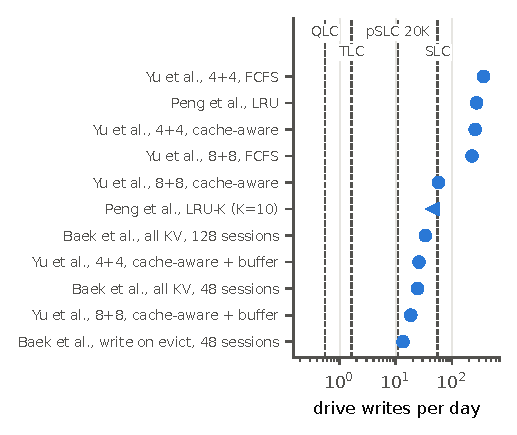
\includegraphics[width=\columnwidth]{fig_demand.pdf}
\caption{Drive writes per day that each published workload puts on its flash, backed out from the reported lifetime, against what each cell type sustains for five years (dashed lines). FCFS is first-come first-served scheduling; 8+8 and 4+4 count HBM and HBF stacks per accelerator; the buffer reserves 10\% of device capacity for cached sessions. The triangle is an upper bound, from a lifetime reported as over six years.}
\label{fig:demand}
\end{figure}

\emph{Published lifetimes.} Solving $L = C\,N/(\mathrm{WAF}\cdot w)$ for $w$, with the capacity, cycles and WAF a paper states, recovers its write rate. Three papers state enough to do this for \RecN{} configurations.\cite{yu2026hbf,baek2026hotcold,peng2026gr} Fig.~\ref{fig:demand} shows the result. The workloads ask for \RecDwpdMin{} to \RecDwpdMax{} drive writes per day, and a five-year SLC stack sustains \DwpdSLC{}. The policy that decides what gets cached moves a workload across the line. In Yu et al., cache-aware scheduling alone cuts the write rate \YuPlainCutMin{}- to \YuPlainCutMax{}-fold against first-come first-served, and adding the capacity buffer cuts it \YuCutMin{}- to \YuCutMax{}-fold.

Li et al.'s result follows from the same identity. They find that a TLC HBF tier lasts 0.56 times as long as a capacity-matched SSD pool, across all four of their traces. Their own budgets, 21.7 and 38.4~TB per day, have exactly that ratio.\cite{li2026hbfsucks}

\emph{What a denser cell changes.} The cell sets the residence time. Table~\ref{tab:identity} gives it for each cell type: from \ResSLCmin{} minutes for SLC to \ResQLCh{} hours for QLC, with TLC at \ResTLCh{} hours. Adding stacks raises the budget, not the residence time. Denser cells keep blocks longer but absorb fewer bytes. At equal die count, SLC can write \RatioTLC{} times more bytes over its life than TLC, so on TLC every published lifetime shrinks by the same factor, and none of the \RecN{} reaches five years. The longest falls to \BaekEvictTLC{} years.

\emph{Retention break-even.} Relaxing retention raises the cycle rating $N$ and nothing else. So each byte ratio above is also the factor by which TLC's cycle rating must grow to write as many bytes. On the same die, TLC needs \SameDieMax{} times more cycles to absorb as many bytes as pSLC rated for 30,000, and \SameDieMin{} times more against a 20,000-cycle pSLC. Luo et al.'s 2.7-fold estimate clears only the second. Against native SLC dies, TLC would need \RatioTLC{} times more.

\section{When KV blocks come back}

Residence time matters only relative to when a block is needed again. We replay each trace through an LRU cache of about 1~TB of HBM, 6,000 Llama-3.1-70B blocks, and record the time from each eviction to the block's next reference. The Qwen-Bailian release holds four two-hour traces from a commercial service.\cite{wang2025kvcachewild} To give every evicted block the same \QwWindowMin{}-minute look-ahead, more than three times SLC's residence, we count only blocks evicted in the first 30 minutes of each trace. We count a reuse even if an earlier block of its prompt is missing, so the shares below are upper bounds.

\begin{figure}[t]
\centering
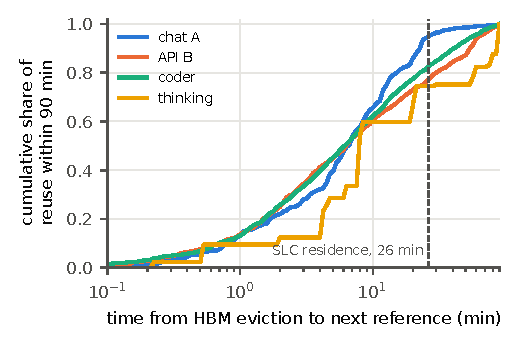
\includegraphics[width=\columnwidth]{fig_gaps_micro.pdf}
\caption{Cumulative share of the reuse seen within \QwWindowMin{} minutes of HBM eviction, for the four two-hour Qwen-Bailian traces. The curves keep rising after SLC's \ResSLCmin{}-minute residence.}
\label{fig:gaps}
\end{figure}

Between \QwReuseMin{}\% and \QwReuseMax{}\% of evicted blocks are referenced again within \QwWindowMin{} minutes, depending on the trace; this is the share an admission policy has to find. Median gaps are \QwMedMin{} to \QwMedMax{} minutes. SLC's residence covers \QwSlcMin{}\% to \QwSlcMax{}\% of the reuse. The remaining \QwAfterMin{}\% to \QwAfterMax{}\% arrives later, when only a denser cell or an SSD pool still holds the block (Fig.~\ref{fig:gaps}).

Longer gaps come from people returning to a conversation. In \WcFollowUps{} follow-up turns from the WildChat dataset,\cite{zhao2024wildchat} measured in our earlier work,\cite{nikzat2026roar} the median gap between turns is \WcMedianS{} seconds. Still, \WcOverOneH{}\% of follow-ups come more than an hour later, and \WcOverTLC{}\% after TLC's \ResTLCh{}-hour residence.

\section{What flash adds in a serving node}

Residence times and budgets ignore what decides real deployments: prefix dependence, policies that must guess which blocks will return, finite flash capacity, and host DRAM in front of flash. We simulate the hierarchy of Fig.~\ref{fig:tiers} with our open KV-cache simulator,\cite{nikzat2026roar} to which we added a host-DRAM tier. The metric is GPU-hours saved per day: accelerator time not spent recomputing cached prompt blocks, on a node with \SimNodeGPUh{} GPU-hours per day.

\emph{Workload.} We know of no public trace with prefix hashes that spans a day, so we construct two-day workloads. Mooncake's public tool-and-agent trace covers one hour.\cite{qin2025mooncake} We replay it 48 times. Each replay keeps a request with a probability that follows a daily load curve between 0.3 and 1.0, and renames every block, so no prompt prefix is shared across hours. Each request is then issued again, with probability \WcReturnPct{}\%, after a gap drawn from the WildChat gaps over an hour. The \WcReturnPct{}\% counts all WildChat turns, including last turns; among turns that get a follow-up it is the \WcOverOneH{}\% given above. We call these re-issued requests late returns. Day~1 warms the caches, and day~2 is measured. We repeat the main runs with Mooncake's conversation hour, and with two more random seeds for the request sampling.

\emph{Hierarchy and flash.} HBM holds about 1~TB of KV state under LRU. Blocks it evicts enter a first-in, first-out host-DRAM buffer of 1~TB; we also try none, 2~TB and 4~TB. An NVIDIA DGX B200 node ships with 2~TB of host memory and supports 4~TB. Blocks leaving DRAM go to the flash admission policy. A flash hit saves the block's recomputation time at its depth in the prompt, minus the flash read time. Flash is eight stacks, one per GPU, with the five-year budget of Eq.~\eqref{eq:budget} at equal die count, so every policy for a cell type has the same writable bytes. The SSD alternative is Yu et al.'s 32 drives of 1~TB, rated here for 3~DWPD.

\emph{Policies.} \emph{Write within budget} writes every block that leaves DRAM until the minute's share of the budget is used. \emph{Admit on second reference} does the same for blocks seen at least twice. \emph{Adaptive $k$} admits blocks seen at least $k$ times and adjusts $k$ to stay on budget. \emph{ROAR} (read-often, append-rarely), our earlier policy, writes a block when its estimated saving exceeds a price on wear that rises when writes run ahead of schedule.\cite{nikzat2026roar} Both online controllers keep the settings of our earlier work; we did not retune them for these traces. Adaptive $k$ stays within \SimAkOverMax{}\% of its budget. ROAR can overshoot: by up to \SimRoarOverShown{}\% in Table~\ref{tab:sim} and Fig.~\ref{fig:value}, and by \SimRoarOverMax{}\% in one other DeepSeek-V3 run. The \emph{oracle} knows the future and picks the blocks with the largest savings, with half the online policies' write allowance. The bound is \emph{unlimited flash}: every block leaving DRAM is written to flash with no capacity or wear limit.

\begin{table*}[t]
\caption{GPU-hours saved per day by flash hits on day~2 of the constructed tool-and-agent workload: eight-GPU node (\SimNodeGPUh{} GPU-hours per day), 1~TB of host DRAM, five-year budgets at equal die count. Within a column, every online policy has the same writable bytes; the oracle has half. pSLC is rated for 20,000 cycles. Bold: best online policy within 5\% of its budget. *: more than 5\% over budget. --: not run.}
\label{tab:sim}
\centering\footnotesize
\begin{tabular}{@{}lrrrrrrrr@{}}
\toprule
 & \multicolumn{4}{c}{Llama-3.1-70B} & \multicolumn{4}{c}{DeepSeek-V3 KV format} \\
\cmidrule(lr){2-5}\cmidrule(lr){6-9}
Policy & SLC & pSLC & TLC & SSD pool & SLC & pSLC & TLC & SSD pool \\
\midrule
\tabinput{tab_sim_micro.tex}
\bottomrule
\end{tabular}
\end{table*}

\begin{figure}[t]
\centering
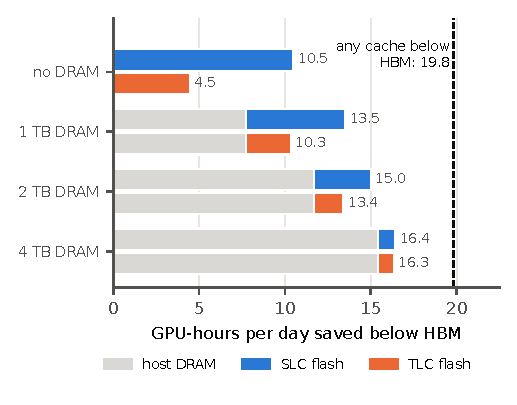
\includegraphics[width=\columnwidth]{fig_value.pdf}
\caption{GPU-hours per day saved below HBM by host DRAM (gray) and by eight SLC or TLC stacks behind it (ROAR), Llama-3.1-70B. The dashed line is what an unlimited cache below HBM saves. At 4~TB, ROAR's SLC run is \SimDramFourRoarOverPct{}\% over budget; on budget, adaptive $k$ saves \SimDramFourAkSLC{} on SLC.}
\label{fig:value}
\end{figure}

Table~\ref{tab:sim} and Fig.~\ref{fig:value} give the results. Five findings follow.

\emph{Host DRAM takes most of the value.} An unlimited cache below HBM would save \SimCeilZero{} GPU-hours per day (Fig.~\ref{fig:value}). Host DRAM alone recovers \SimDramShareOne{}\% of that with 1~TB and \SimDramShareFour{}\% with 4~TB. Eight SLC stacks without DRAM recover \SimNoDramSlcShare{}\%. Behind 4~TB of DRAM, no flash tier of any size can add more than \SimCeilFour{} GPU-hours per day, \SimCeilFourPct{}\% of the node. SLC and TLC each add about one. What DRAM leaves behind is reuse after long gaps. With four times the measured late returns, 4~TB of DRAM recovers only \SimXFourDramShareFour{}\%, and flash could still add up to \SimXFourCeilFour{} GPU-hours per day. There TLC adds more than SLC: \SimXFourFourTLC{} against \SimXFourFourSLC{} with adaptive $k$.

\emph{Behind 1~TB of DRAM, SLC wins for Llama-3.1-70B, by less than its byte advantage.} With ROAR, SLC saves \SimRoarSLC{} GPU-hours per day, \SimRoarSlcCeilPct{}\% of the \SimCeilOne{} that unlimited flash would, and TLC \SimRoarTLC{}. SLC writes \RatioTLC{} times more bytes, yet saves \SimSlcOverTlc{} times as much, because each extra byte is worth less: a block SLC writes earns \SimHitsPerBlockSLC{} hits, one TLC writes \SimHitsPerBlockTLC{}. Late returns favor TLC. With none, TLC saves \SimRetXZeroTLC{} GPU-hours per day; at four times the measured rate, \SimRetXFourTLC{}. SLC moves only from \SimRetXZeroSLC{} to \SimRetXFourSLC{}. At sixteen times the rate, the two tie (\SimRetXSixteenSLC{} and \SimRetXSixteenTLC{} with adaptive $k$). On the same die, pSLC at 20,000 cycles beats TLC by \SimPslcOverTlcAkPct{}\% with adaptive $k$, which stays on budget. With Luo et al.'s 2.7-fold cycle gain, TLC saves \SimRelaxTlcL{}, slightly more than pSLC at 30,000 cycles (\SimPslcHighL{}). So TLC matches pSLC in saved GPU time with less than the \SameDieMax{}-fold cycle gain it would need to write as many bytes.

\emph{The reusable write rate decides the cell type.} We define it as the bytes per day that leave DRAM and will be read again, which is what the oracle writes when wear does not bind. For Llama-3.1-70B it is \SimReusableL{}~TB per day: \SimReusableLOverTLC{} times TLC's budget, so TLC must drop reusable blocks, but only \SimReusableLOverSLCPct{}\% of SLC's. DeepSeek-V3's compact KV format gives \SimReusableDS{}~TB per day, \SimReusableDSOverTLCPct{}\% of TLC's budget, so no cell is wear-limited. In the busiest trace hour, one terabyte of DRAM also holds a DeepSeek-V3 block for about \DramResDSmin{} minutes, against \DramResLs{} seconds for Llama-3.1-70B. With perfect knowledge, the cell type then makes no difference: the oracle saves \SimDsOracleMin{} to \SimDsOracleMax{} on every cell, nearly the \SimCeilDS{} of unlimited flash. Online, across three seeds, the best policy saves \SimSeedDsSlcRange{} GPU-hours per day on SLC and \SimSeedDsTlcRange{} on TLC. The policies that pace writes to the wear budget, write within budget, adaptive $k$ and ROAR, do worst on SLC. Wear never binds there, so they write nearly every block and fill the stack, which then holds each block for about \SimDsSlcResMin{} minutes.

\emph{An SSD pool is a strong alternative.} The pool holds more than eight stacks of any cell type, and its budget keeps each block for about \SsdResThreeH{} hours. An SSD hit, at \TDramMs{}~ms over PCIe, is still worth \SimSsdHitValuePct{}\% of an HBF hit. With the pool, ROAR saves \SimRoarSSD{} GPU-hours per day for Llama-3.1-70B, close to SLC, and the oracle saves \SimOracleSSD{}, more than on SLC. For DeepSeek-V3, adaptive $k$, which stays on budget, saves \SimSeedDsSsdAkRange{} on the pool across seeds, more than twice the best online policy on any HBF cell type.

\emph{Choosing what to write matters as much as the cell.} Writing everything within the budget saves \SimWaSLC{} GPU-hours per day on SLC but only \SimWaTLC{} on TLC, where the small budget goes to blocks that never return. The oracle reaches \SimOracleSlcCeilPct{}\% of the unlimited-flash ceiling on SLC, against ROAR's \SimRoarSlcCeilPct{}\%; predicting reuse is the largest gap left. ROAR leads adaptive $k$ by \SimRoarOverAkMin{}\% to \SimRoarOverAkMax{}\% for Llama-3.1-70B but not for DeepSeek-V3.

For Llama-3.1-70B, these results hold across seeds: ROAR's savings vary by at most \SimSeedSpreadMax{}\%, and SLC saves \SimSeedRatioRange{} times as much as TLC in every seed. On Mooncake's conversation hour, SLC and TLC save \SimConvRoarSLC{} and \SimConvRoarTLC{}. Doubling the WAF halves every budget but lowers savings by only \SimWafTwoDropRangeSLC{}\% on SLC and \SimWafTwoDropRangeTLC{}\% on TLC (ROAR and adaptive $k$).

\section{Limitations}

The simulator measures GPU time saved, not time to first token or throughput at a latency target. It credits a DRAM hit with the full recomputation time and ignores the \TDramMs{}~ms transfer, which overstates DRAM's savings by about \DramBiasPct{}\%; DRAM hits use \SimDramLinkPctOne{}--\SimDramLinkPctFour{}\% of one PCIe link on average. The workload is constructed from one-hour traces, and renaming blocks each hour removes reuse of shared prefixes across hours except through late returns. The cycle ratings are industry figures for SSD-class dies, not HBF measurements; error correction, read-disturb repair and temperature are not modeled. For DeepSeek-V3 we model only its KV format; its weights would not fit beside 1~TB of KV state on one eight-GPU node. HBF is modeled as added to HBM, not replacing it, which favors HBF. Equal die count is not equal cost, and the SSD pool holds more bytes than the HBF tier. We could not compare at equal cost because HBF prices are not public.

\section{What HBF designers should do}

\emph{Size host DRAM first.} It serves short gaps without wear, and each terabyte lowers what flash can add. Behind a large DRAM tier, flash serves only long gaps; when those are common, as at four times the measured rate, TLC beats SLC.

\emph{Measure the reusable write rate after DRAM and compare it with each cell's budget.} If it exceeds a dense cell's budget but not SLC's, as for Llama-3.1-70B, SLC wins. If it fits every budget, as for DeepSeek-V3's compact format, capacity decides, and the largest tier, often an SSD pool, wins. Compact KV formats and KV quantization move a workload toward the second case. When wear does not bind, admit on reuse, not on a wear price.

\emph{Spend effort on predicting reuse.} The gap between online policies and the oracle is larger than most differences between cell types.

\emph{Compare against the SSD pool the node already has}, at equal cost once HBF prices are known.

\emph{Measure cycle ratings on current 3D NAND at retention targets of days.} On the same die, a gain near Luo et al.'s estimate for 3D NAND, 2.7 times, decides between pSLC and TLC.

\emph{Report lifetime claims with the inputs in Table~\ref{tab:checklist}.} The comparison in Fig.~\ref{fig:demand} was possible only for papers that stated them.

\begin{table}[t]
\caption{What an HBF lifetime claim should report.}
\label{tab:checklist}
\centering\footnotesize
\begin{tabular}{@{}>{\raggedright\arraybackslash}p{2.6cm}>{\raggedright\arraybackslash}p{5.1cm}@{}}
\toprule
Item & Why \\
\midrule
Cell type, die model, cycle rating & set residence and budget (Eqs.~\ref{eq:budget} and~\ref{eq:residence}) \\
Retention target & a weaker target changes the cycle rating \\
Capacity that absorbs writes & usable KV capacity, not stack capacity \\
WAF and its source & lifetime scales inversely with it \\
Write rate and its source & trace, load scaling, hours measured \\
Scheduling and admission policy & either can change the write rate tenfold \\
KV bytes per token & model and KV format change it severalfold \\
Other tiers modeled & host DRAM and SSDs set what flash adds \\
Lifetime in DWPD & comparable with SSDs and other papers \\
\bottomrule
\end{tabular}
\end{table}

\bibliographystyle{IEEEtran}
\bibliography{refs_micro}

\begin{IEEEbiographynophoto}{H. R. J. Nikzat}
is an undergraduate student at Bates College, Lewiston, ME 04240, USA. His research interests include memory hierarchies for LLM inference, flash endurance, and GPU simulation of cold-atom physics. Contact him at rnikzat@bates.edu.
\end{IEEEbiographynophoto}

\end{document}
